% !TEX TS-program = pdflatex
% !TEX encoding = UTF-8 Unicode

\documentclass[sigconf]{acmart}
\captionsetup{font=footnotesize}
\usepackage{graphicx}

\settopmatter{printacmref=false} % Removes citation information below abstract
\renewcommand\footnotetextcopyrightpermission[1]{} % removes footnote with conference information in first column
%%\pagestyle{plain} % removes running headers
\thispagestyle{empty}
%%
%% \BibTeX command to typeset BibTeX logo in the docs
\AtBeginDocument{%
    \providecommand\BibTeX{{%
        \normalfont B\kern-0.5em{\scshape i\kern-0.25em b}\kern-0.8em\TeX}}}

\setcopyright{none}
\copyrightyear{}
\acmYear{}
\acmDOI{}

\acmConference[Computer Science]{}{University of Salerno}{UNISA}
\acmBooktitle{Real time Alexa packets profiling analysis}
\acmPrice{}
\acmISBN{}

\begin{document}

    \title{Real time Alexa packets profiling analysis}


    \author{Giuseppe Polese}
    \orcid{0000-0002-8496-2658}
    \email{gpolese@unisa.it}
    \affiliation{
        \institution{Universit\'a degli studi di Salerno}
        \streetaddress{}
        \city{Salerno}
        \state{}
        \country{Italy}
        \postcode{}
    }

    \author{Bernardo Breve}
    \orcid{0000-0002-3898-7512}
    \email{bbreve@unisa.it}
    \author{Stefano Cirillo}
    \orcid{0000-0003-0201-2753}
    \email{scirillo@unisa.it}
    \affiliation{%
        \institution{Universit\'a degli studi di Salerno}
        \streetaddress{}
        \city{Salerno}
        \state{}
        \country{Italy}
        \postcode{}
    }

    \author{Biagio Boi}
    \email{b.boi@studenti.unisa.it}
    \affiliation{
        \institution{Universit\'a degli studi di Salerno}
        \streetaddress{}
        \city{Salerno}
        \state{}
        \country{Italy}
        \postcode{}
    }

    \begin{abstract}
        Nowadays, the introduction of home virtual assistents like Alexa Echo or Google Home became a practice, just considering that over 27\% of families owns one.

        It's obvious that those devices simplify the life by creating a smart house with few money; but what's the impact these devices have on people's privacy?
        There are a lot of cases in the United States in which the judge asked to Amazon to provide the recording done by the Echo in order to find helpful
        evidences for the case; so, the question is: "It's possible to prevent the sending of sensible informations to the servers when the wake word is not pronunced?"

        In this project we will profile each packet exchanged between the Alexa Echo and the Server in order to classify the nature of the packets and consequentially we will use a machine learning model to discover if exists a clear correlation between the characteristics of the packet and the classification done.
    \end{abstract}

    \keywords{data analytics, alexa, packets profiling}


    \begin{teaserfigure}
        \rule{\linewidth}{1mm}
%%  \includegraphics[width=\textwidth]{sampleteaser}
%%  \caption{Insert text here}
%%  \Description{insert description here}
%%  \label{fig:teaser}
    \end{teaserfigure}

%%
%% This command processes the author and affiliation and title
%% information and builds the first part of the formatted document.
    \maketitle


    \section{Introduction}
    The evolution of smart devices over last years has increased exponentially and the introduction of these devices within the house is progressively growing.
    The major problem related to these devices is that usually the privacy is not considered, although there are a lot of regulations (just see the GDPR) that describe how the user data have to be stored and who can access to these data.
    Starting from these two points I decided to understand what happens within the context of smart assistance device such as Alexa Echo.
    Reading on the Amazon Alexa website it's clear how and when they send data to the Amazon Cloud, but in opposition we have some cases in which the recording done by the Echo have been used during the processes in order to extract some evidence.
    In order to clarify this aspect and the role of the smart assistance devices I decided to analyze the outgoing traffic from the device and classify it by considering the environmental conditions.
    The first phase of this analysis consist in understand which kind of packets are sent from the device in order to create a complete dataset of packets sent by the device; during the second phase I try to understand if exist a pattern that identify the packets that souldn't be sent to the Cloud by creating a machine learning model able to identify them.


    \section{State of Art}
    During the last years different research have been done, related to different aspects of the security and privacy within the IoT context.
    F. Z. Berrehili and A. Belmekki \cite{berrehili} have done a study on the Privacy Preservation in the IoT context that shows all the risks directly related to the architecture; in particular, it underlines the need to always guarantee the anonymization of sensibile data by hidding the correlation between the data itself and the person who produced these data (that is also one of the principle of GDPR).
    Despite these studies, there is an huge percentage of devices that do not consider as serious all the aspects related to the privacy, in particular J. Liu and W. Sun \cite{liu} show different attacks againit werables devices at different levels of the ISO/OSI stack and considering different aspects of privacy and security like data integrity, authentication, authroization, etc. The study shows a lot of attacks aim at sniff the packets during the communication in order to collect sensible informations; this seems to be caused from the problem related to the poor encryption mechanisms implemented into the smart devices.


    \section{Alexa architecture \& security}
    The Alexa architecture isn't easy to explain, we will resume the keypoint in order to better understand the main functionalities for our purpose.
    \begin{enumerate}
        \item Alexa is always in listening waiting for the wake word to be pronunced to start the recording of the voice;
        \item From the wake word, till the end of commands, Alexa will record the speech and partially sends it to Alexa Voice Service, that can be considered as the brain of Alexa;
        \item Alexa Voice Service will process the audio using Natural Language Processing and Natural Language Understanding in order to retrieve a response for the given request.
        \begin{enumerate}
            \item Natural Language Processing (NLP) improve the Word Segmentation that separate a chunk of continuous text into separate words.
            \item Natural Language Understanding (NLU) is a subtopic of NLP and uses the AI to map text to the meaning\cite{NLU} in order to understand the speech and the request.
        \end{enumerate}
        \item Depending on the sent command, the Voice Service will take an action (turn on the light) or send the information back to the device and Alexa may speech.
    \end{enumerate}
    All the communications between the Echo and the Server are secured by using an SSL/TLS encryption schema.
    More throughly, the Echo looks for an available Amazon Server each 2 minutes and then establish a connection (by following the SSL Handshake).
    Once the communication has been initialized it starts to send different encrypted packets of different size; clearly, these pakcets may contains both authorized and unauthorized data.
    It may be important to underline that all the recordings are available on the Amazon platform and can be reproduced and deleted whenever the user wants only by accessing to the platform and this guarantee more transparency to the user that can directly handle all the recordings.
    The point is that here we found only the recordings done by the Echo in an authorized way (when the wake word it's been pronounced), but this doesn't imply that some other recordings can exist and be stored in hidden way.


    \section{Packets analysis}
    In order to analyze the packets we need to create some kind of proxy between the Echo and the Router (that will send the packets to the server); for this reason the Echo it's connected directly to the computer using the Windows mobile hotspot.

    \subsection{Python script}
    The step described above is necessary since we need to execute a python script on the same machine that recieve the packets from the Echo. In particular, the script will intercept every packet sent by the Echo using PyShark library, that is a library developed in python based on the software Wireshark, able to intercept every kind of packet and retrieve useful information about them. The first step before to use the library is to configure it by setting up the preferred virtual network card (in our case will be that on which is run the hotspot) and the device we want to sniff the packets. Once these two parameters have been declared, the sniffing can start: we will collect only those packets sent by the Echo, by discarding the others (those recieved from the Server); this choice it's been taken since we don't want to block or discover anything about the recieved packets, we want only to block those packets that shouldn't be sent. A simple python function is called every time a new packet has been sent, it process the packet by checking at: protocol, flags, content type and length. During the processing phase, the packets are classified and inserted into the relative dataset (one for each context in which the script has been executed). This classification is just relative, a manual phase is necessary in order to detect errors.

    \subsection{Classification}
    Is possible to classify the type of packet by looking at flags, packet size and protocol used.
    There are different types of packet that will later be included in the dataset as classes:
    \begin{enumerate}
        \item \textbf{handshake}: At the beginning of each new SSL/TLS communication between the Echo and the Server there are different packets exchanged in order to establish a secure communication.
        These packets can be easily identified by the protocol used for the communication (TLS) and by checking the flags related to the content of the message, in particular, the possible flags are:
        \begin{enumerate}
            \item Change Cipher (20).
            \item Server Hello - Show Certificate - Encrypted Message (21).
            \item Alert (22).
        \end{enumerate}
        \item \textbf{syn}: Packets with fixed length are sent from the device in a fixed interval, seems that them are used to synchronize the Echo to the Server.
        \item \textbf{ack}: These are the classical packets used to confirm that the received packets are valid and successfully received.
        \item \textbf{retransmit}: These packets are used to retransmit the data that didn't received an ack, usually this happens when the Echo try to communicate with other Amazon devices (Fire Stick for ex.) but doesn't receive response.
        \item \textbf{app\_data}: These packets are relative to the normal communication of the Echo and can be easily recognized since the communication happens over TLS/SSL protocol and by checking the flag of the considered packet that is equal to 23.
        In particular, we will include in this class all the communication packets that include also recording of voice occurred during the conversation between the Echo and the final costumer.
        \item \textbf{not\_relevant}: We will include in this category all packets that don't match any of the other categories, and are not relevant for our study.
    \end{enumerate}
    It may be import to underline that the packets classified as app\_data may include both authorized and not authorized packets.
    The unauthorized packets include all those packets sent in a context in which no application date should be sent to the Server by considering the environmental variables (no wake word pronounced) and hardware aspects (microphone muted by pressing the relative button); for this reason is important to introduce some classes related to these aspects.
    The aim is to distinguish three kind of packets:
    \begin{itemize}
        \item \textbf{not\_justified}: packets sent to the Server in a context in which the Echo is unable to send these data by considering the hardware aspects.
        \item \textbf{justified}: packets sent to the Server without any interaction between the Echo and the Customer, but the Echo is able to listen.
        \item \textbf{expected}: packets sent to the Server since an interaction between the Echo and the Customer happened.
    \end{itemize}
    Clearly, the only allowed packets are those classified as "Expected".
    \subsection[Consideration on packet]{Consideration on packet analysis}
    It's important to do some consideration over the analysis / collection phase just described, in fact there are a lot of behavioural pattern that the Echo follow to perfrom some actions:
    \begin{itemize}
        \item As introduced in the previous section there are some kind of packets that always follow the same schema in a given interval.
        These packets may be sent to guarantee the synchronization with the Amazon Alexa application and with the Amazon servers.
        There are two possible synchronization packets:
        \begin{enumerate}
            \item A packet of 100 byte is sent each 30 seconds (30002 milliseconds)
            \item A packet of 99 byte is sent each 90 seconds (90820 milliseconds)
        \end{enumerate}
        The communication always happens using SSL/TLS, so it's impossible to decrypt the content of these message and confirm that is securely a synchronization packet.
        \item Music stream pattern is dependent on music service used; a stream with Amazon Music always uses a secure connection by using TLS.
        \begin{figure}[h!]
            \centering
            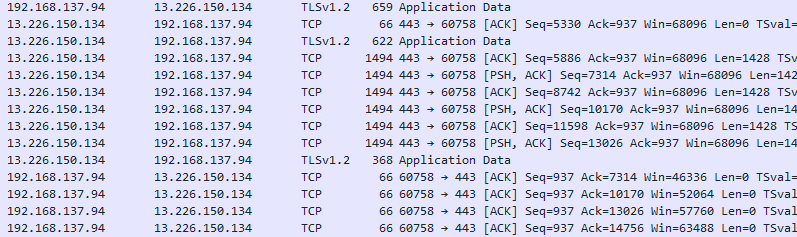
\includegraphics[width=0.8\columnwidth]{img/capture_amazon_music.png}
            \caption{Captured packets during Amazon Music streaming (Wireshark)}
            \label{fig:capture_amazon_music}
        \end{figure}

        Instead, a stream with Spotify makes an HTTP request to Spotify Server that can be captured and replicated
        \begin{figure}[h!]
            \centering
            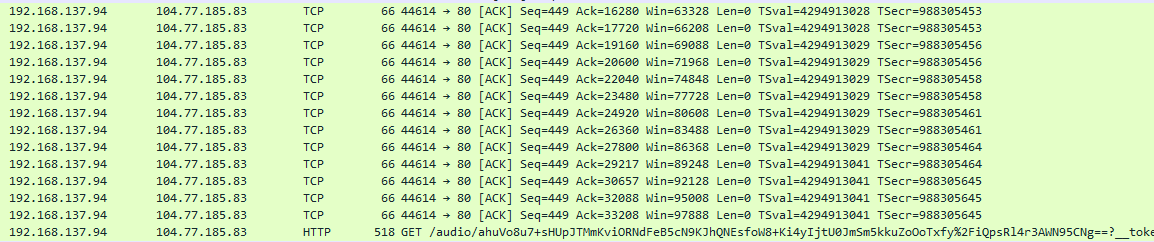
\includegraphics[width=0.8\columnwidth]{img/capture_spotify.png}
            \caption{Captured packets during Spotify streaming (Wireshark)}
            \label{fig:capture_spotify}
        \end{figure}
        \item Echo changes server every 2 minutes, for this reason there are a lot of handshake.
    \end{itemize}


    \section{Dataset}
    In order to create a valid and well-distributed dataset we analyzed the behavior of the Echo in different context, in particular by considering different cases:
    \begin{enumerate}
        \item \textbf{Microphone mute}: when the hardware button is pressed and the device should be unable to send application data to the server.
        \begin{figure}[h!]
            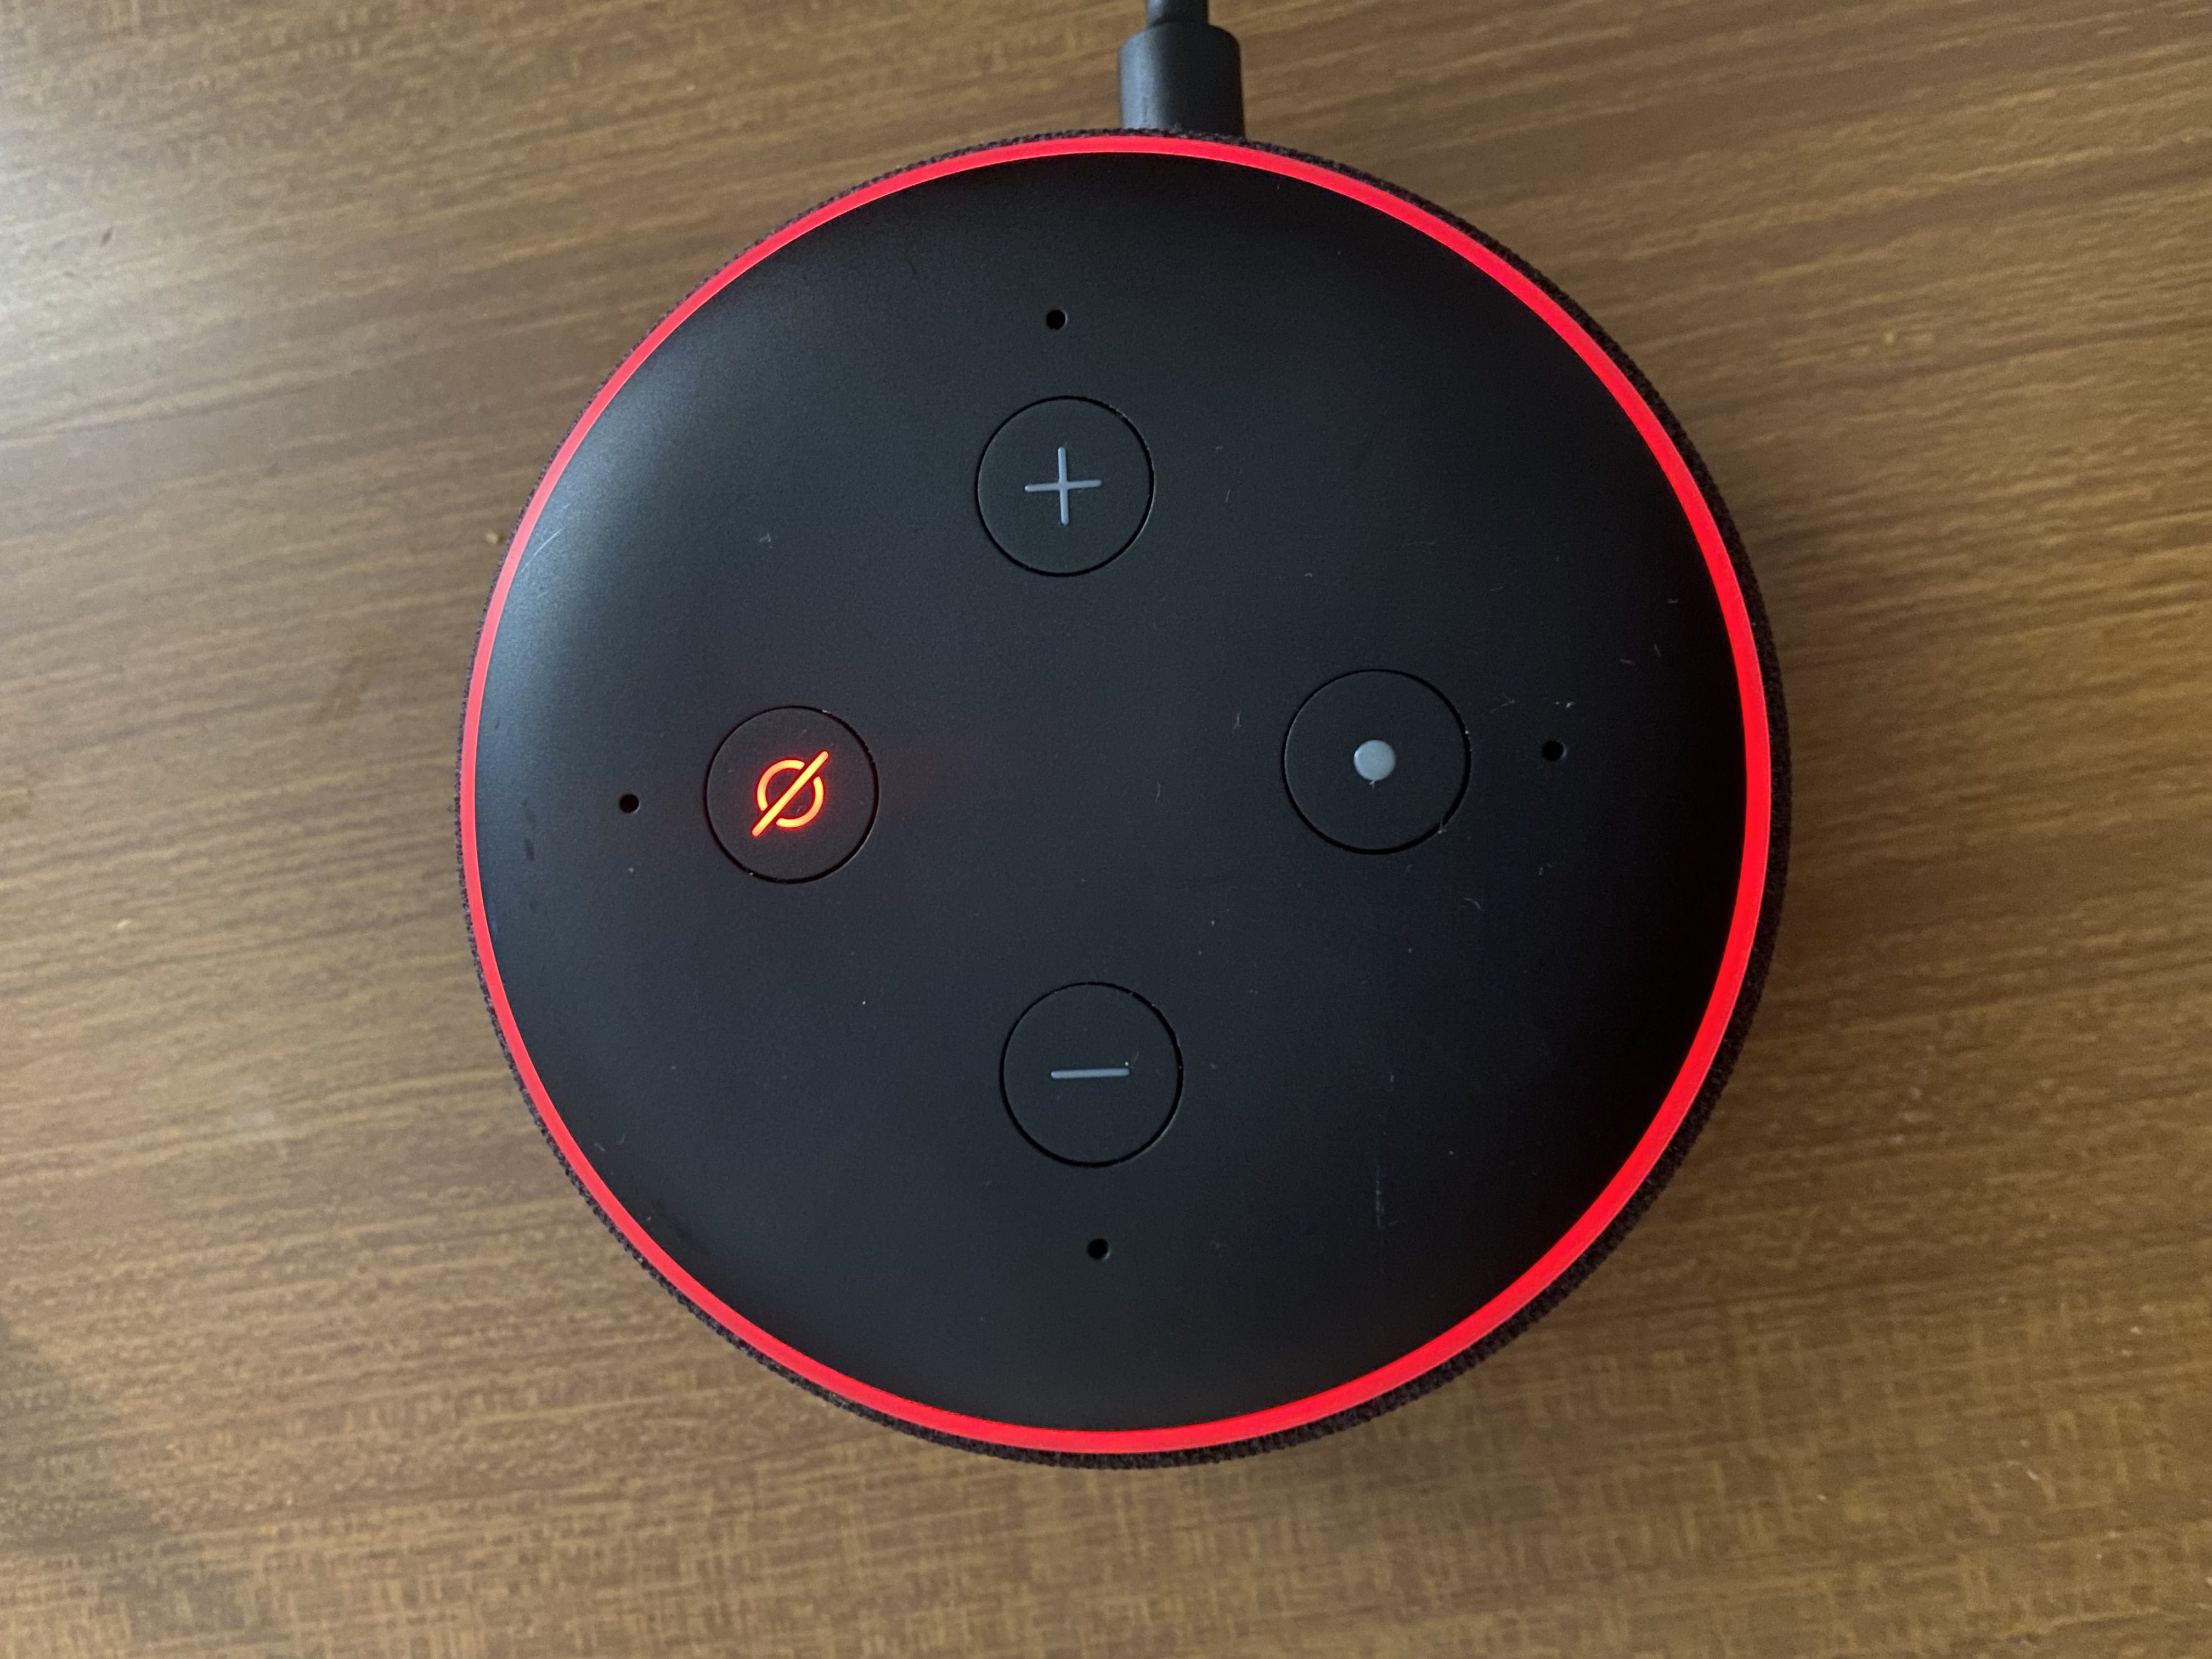
\includegraphics[width=0.8\linewidth]{img/alexa_red.jpg}
            \caption{Echo when the disable microphone button has been pressed.}
            \label{fig:Alexa_red_led}
        \end{figure}
        \item \textbf{No wake word pronounced}: when the device is able to listen the voice but shouldn't send to the Server any packets of application data.
        \item \textbf{Normal stream of data}: when a communication happens.
        It may include different questions or requests, for example:
        \begin{enumerate}
            \item How is the weather today?
            \item When does Liverpool play?
            \item Add milk to the shopping list.
            \item How much is 20 + 20?
        \end{enumerate}
        All these questions or requests expect a response from the Server, so a huge amount of ack will be sent from the device.
        \item \textbf{Streaming}: when the user request for a song and the Echo start to stream it; also in this case a lot of ack packets are sent from the device as response to the fragment of the item to stream (a song for example).
    \end{enumerate}

    \subsection{Features}
    As introduced in the previous section it's important to collect features related to both hardware and software aspects; let's see in detail which are the considered features with the related meaning:
    \begin{enumerate}
        \item \textbf{date}: the date in which the packet has been collected, in the format YYYY-MM-DD hh:mm:ss:ms;
        \item \textbf{length}: the length of the packet, it includes just the payload (in case of ack packest it's equal to zero);
        \item \textbf{dstip}: the destination ip, collected to analyze the owner of the server to which the packet is directed;
        \item \textbf{dstport}: the destination port;
        \item \textbf{highest\_layer}: the protocol used, in order to parse the protocol into an integer we will use the following mapping:
        \begin{itemize}
            \item 0 - SSL
            \item 1 - TCP
            \item 2 - DATA
            \item 3 - HTTP
        \end{itemize}
        Notice that all the packets that use other protocol are discarded since them have no meaning for our purpose;
        \item \textbf{delta}: the time occured from the previous packet of the same stream;
        \item \textbf{ack\_flag}: the acknowledge flag; it is equal to 1 if the packet contains an ack;
        \item \textbf{microphone}: the status of the microphone, it is equal to 1 if the microphone is active, 0 otherwise;
        \item \textbf{content\_type}: the type of content sent, it is valorized only if the packet is sent over SSL;
        \item \textbf{synchronized}: status of sychronization of the device, it is equal to 1 if the Echo has been previously associated to an account, 0 otherwise.
    \end{enumerate}
    Since we want to map every kind of packet in a class, 8 classes have been declared: handshake, syn, ack, retransmit, not\_relevant, justified, not\_justified and expected.

    \subsection{Dataset merging}
    Since we have collected packets into four different contexts is necessary to merge together all these dataset before to apply any kind of manipulation on data. In particular during the collection phase we have collected 5436 packets when the microphone has been disabled, 39793 packets when the music was streaming (indipendently by the service used), 9374 packets when no wake word has been pronounced and 8027 packets during a normal conversation with the Echo. Clearly, a first overview on these numbers may start thinking that it's totally unbalanced; but we should remember that during the streaming of contents there is an huge amount of ack packets that can be potentially discarded; we will see this operation in the following subsection.

    \subsection{Avoid NaN values}
    During a first overview on collected packets it's been noticed that there are some packets in which the content\_type feature is set to NaN.
    \begin{figure}[h!]
        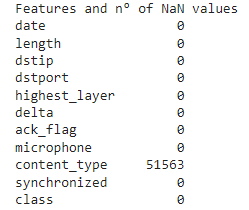
\includegraphics[width=0.8\linewidth]{img/nan_values.png}
        \caption{NaN values related to the content\_type feature.}
        \label{fig:nan_values}
    \end{figure}
    This problem has been caused by the collecting phase; in fact, as already introduced in the subsection 5.1, this feature is valorized only when we capture an SSL packet, otherwise it is set to NaN. In order to fix this problem, all the existing NaN values for the content\_type feature has been set to 0.0.

    \subsection{Not relevant features}
    The dataset contains also instance-specific information, like date and destination ip of the pakcets. Since these values cannot be used during the training phase (otherwise the model will use these values to predict the class of the packets) we need to complitely discard these features by deleting the column from the dataset.

    \subsection{Dataset analysis}
    After removed the NaN values and the not relevant features is important to analyze the collected packets in order to understand if them can be already used or exist some other correction that must be applied before the training. The analysis is divided into target and features analysis.

    \subsubsection{Target class analysis}
    Let's start the analysis of the target class by understanding how many packets have been collected for each class.
    \begin{figure}[h!]
        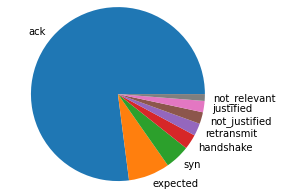
\includegraphics[width=0.8\linewidth]{img/target_class_distribution.png}
        \caption{Distribution of target classes.}
        \label{fig:target_class_distribution}
    \end{figure}

    It's clear the presence of too many ack packets respect to the other classes; as said before this is caused by the streaming context; in fact when a song is streaming, the Echo will send a lot of ack corresponding to each fraction of the song that has been recieved from the Echo. The total amount of ack packets is 48252, respect to: 4813 for expected; 2888 for syn; 1751 for handshake; 1457 for retransmit; 1361 for not\_justified; 1316 for justified and 792 for not\_relevant. Translated into percentage, the number of ack packets correspond to the 77\% over the total. In order to make more balanced the overall dataset we will consider just the 5\% of these packets, that is equal to 2413. The deletion of the row is random.
    \begin{figure}[h!]
        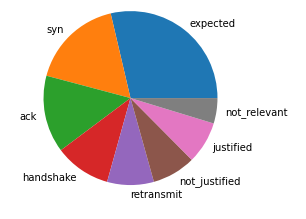
\includegraphics[width=0.8\linewidth]{img/target_class_distribution_after_del.png}
        \caption{Distribution of target classes after 95\% ack packets delete.}
        \label{fig:target_class_distribution_after_del}
    \end{figure}

    \subsubsection{Features analysis}
    After guarantee a good distribution for the target classes, we start our analysis on the features. Let's see the distribution of length of packets in correlation with the target classes.
    \begin{figure}[h!]
        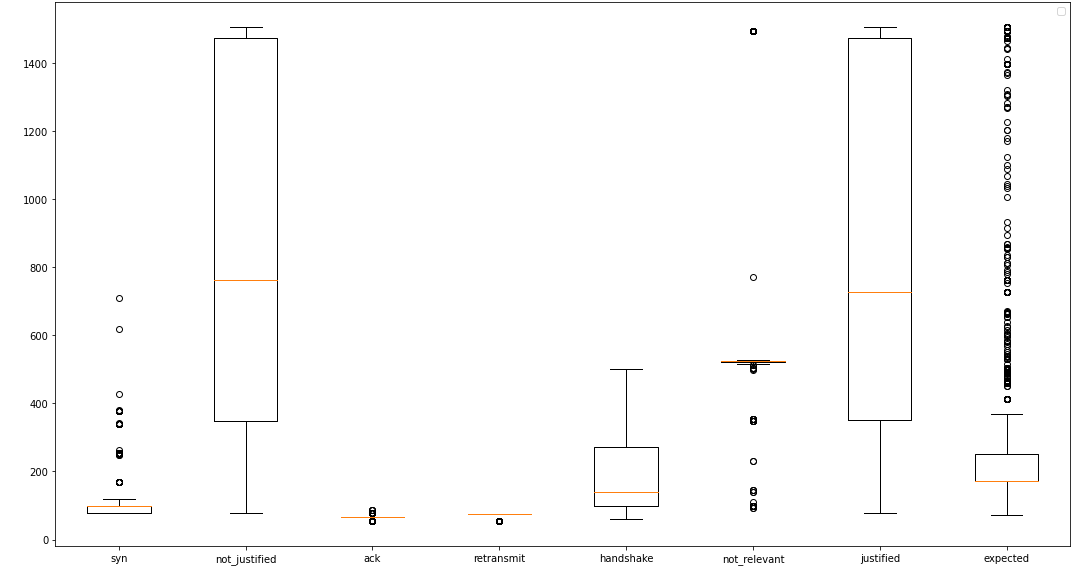
\includegraphics[width=0.8\linewidth]{img/length_distribution.png}
        \caption{Distribution of length in correlation with target classes.}
        \label{fig:length_distribution}
    \end{figure}

    It's clear that synchronization and acknowledge packets have a short length compared with the others; in fact these packets have small data within them, a simple text or just a flag.
    Instead, application data packets such as not justified, justified and expected packets have a variable longer length; in fact these packets are usually used to send voice recording for example.
    A more detailed view of the length of these packets can be seen by plotting the length grouped by the category.
    \begin{figure}[h!]
        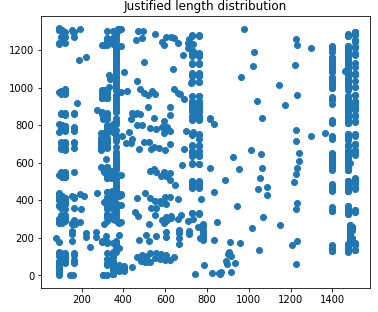
\includegraphics[width=0.8\linewidth]{img/justified_distribution.png}
        \caption{Distribution of length of justified packets.}
        \label{fig:justified_distribution}
    \end{figure}
    \begin{figure}[h!]
        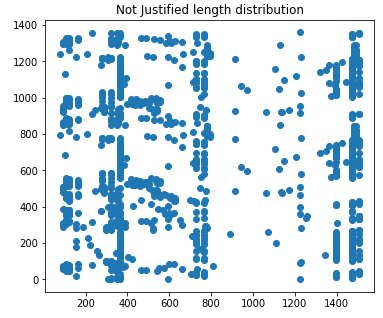
\includegraphics[width=0.8\linewidth]{img/not_justified_distribution.png}
        \caption{Distribution of length of not justified packets.}
        \label{fig:not_justified_distribution}
    \end{figure}
    \begin{figure}[h!]
        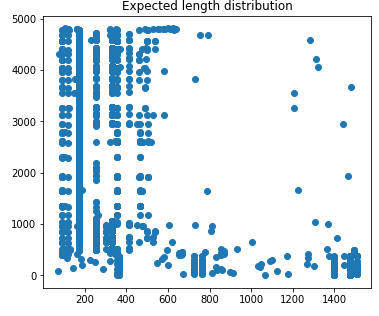
\includegraphics[width=0.8\linewidth]{img/expected_distribution.png}
        \caption{Distribution of length of expected packets.}
        \label{fig:expected_distribution}
    \end{figure}

    Another important consideration is that there is a small difference between the expected and the justified / not justified packets; the first ones usually have a smaller length, while the others have similar behaviour between each other but the average of length is much higher respect to the expected ones.
    Anyway we are not worried about the difficulty for the classifier to distinguish the justified ones from the not justified ones; in fact we know that any justified packet exists with the microphone off (by the assumption done during the collection phase).

    Notice that this behaviour is not exclusive each other, in fact some not justified packet may exists when the microphone is on and nothing is happening in the external environment.
    \begin{figure}[h!]
        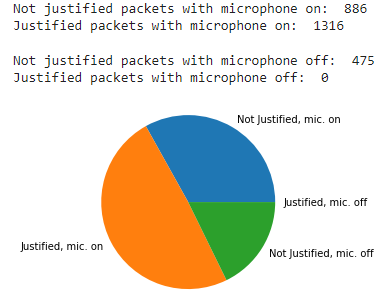
\includegraphics[width=0.8\linewidth]{img/justified_not_justified.png}
        \caption{Distribution of justified and not justified packets in correlation with microphone on/off.}
        \label{fig:justified_not_justified}
    \end{figure}



    Till now, we did not talk about the synchronized feature; this feature figure out the state of synchronization of the device (if it is associated with an Amazon account or not). The problem here is that an Echo cannot work if it is not synchronized with any account, in fact if we plot a pie chart of the distribution of this feature we can easily see that all the captured packets have been captured when the device was synchronized.
    \begin{figure}[h!]
        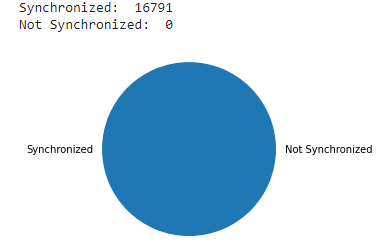
\includegraphics[width=0.8\linewidth]{img/syn_not_syn.png}
        \caption{Distribution of synchronized packets.}
        \label{fig:syn_not_syn}
    \end{figure}

    For this reason we have to delete also this feature (it isn't relevant for our purpose). One of the last analysis regards the distribution of ack flag; in fact this flag seems quite always set to 1 (usually a communication packets may contains also an acknowledge of the previous recieved packet) but we decide to mantain this feature since there is a 10\% of packets in which this flag is set to 0, so it is useful for the training.


    \begin{figure}[h!]
        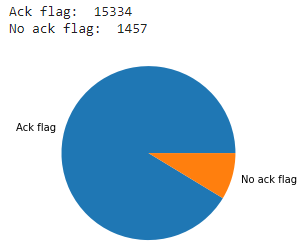
\includegraphics[width=0.8\linewidth]{img/ack_no_ack.png}
        \caption{Distribution of ack packets.}
        \label{fig:ack_not_ack}
    \end{figure}

    Last analysis regard the distribution of highest\_layer feature. Here we have a lot of SSL packets because this is the major protocol used for the communication between the Echo and the Server; while TCP protocol is used for the acknowledge packets and the others (data and http) are used only when a song is requested to the spotify server or for others synchronization features.
    \begin{figure}[h!]
        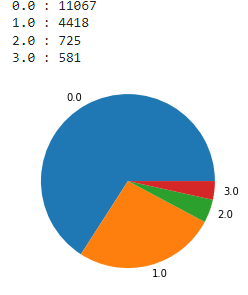
\includegraphics[width=0.6\linewidth]{img/highest_layer.png}
        \caption{Distribution of highest layer.}
        \label{fig:highest_layer}
    \end{figure}


    \section{Machine learning}
    Once the analysis of the dataset is ended we can start the study of the machine learning approaches in order to retrieve which is more suitable for our purpose.

    \subsection{Data balancing}
    Before normalizing the data and apply other machine learning techniques we need to balance the dataset; as we have seen in the previous section there is a small unbalancing between expected and synchronization packets respect to the others; for this reason we will apply a SMOTE (Synthetic Minority Oversampling Technique) in order to oversample the packets of the minority classes. SMOTE will repeat the oversampling procedure till the minority classes will reach the proportion of the majority classes. After SMOTE applied, we have a dataset composed by 4813 packets for each class.

    \subsection{Dataset splitting and standardization}
    Once we have balanced the dataset, we need to split it into testing and training dataset. The splitting is done by using the \textit{train\_test\_split} technique, which is implemented into the sklearn library and split the dataset using a randomic approach by starting from test\_size and random\_state parameter. For our purpose we set the test\_size to 0.3, which means the 30\% over the total and random\_state equal to 6. After that the splitting is completed, we need to standardize the existing values in order to normally distribute them, in particular a standard scaler has been applied.

    \subsection{Features evaluation}
    As we will see below, the feature evaluation it's been done by applying a random forest classifier (which fits better for our purpose) and then by analyzing the \textit{feature\_importances} attribute of the classifier.
    \begin{figure}[h!]
        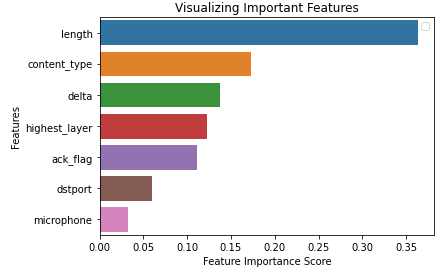
\includegraphics[width=\linewidth]{img/important_features.png}
        \caption{Report of features evaluation.}
        \label{fig:important_features}
    \end{figure}
The report shows that the length it's the most useful feature of the overall dataset as we did previously see during the analysis phase of the project; in fact it depends on the kind of packet, meaning that there is a clear correlation between each other. The second important feature is the content type, that is useful to distinguish the application data from the hanshake packets.
A further important result highlited from this graph is the low importance of ack flag, this because there are a lot of packets classified as application data that have the ack flag equal to 1 (due to architecture of TLS communication which implies the existence of an ack packet together with the application data) that makes difficult for the classifier understand which are the simple ack packets and which are application data ones.

    \subsection{Multiclass classification}
    Since we need to classify instances into one of eight classes we need a multiclass classification, let's see in a more detailed way the possible strategies.

    \subsubsection{Trasformation to binary}
    One possible strategy is to transform the problem of multiclass classification to multiple binary classification problems; this transformation can be done in two ways.

    \textbf{One-vs-rest}: we will create a single classifier for each class and the output will be a real-valued confidence score for its decision. The \textit{sklearn.multiclass} library will help us with the creation of this classifier; in particular the class OneVsRestClassifier will create a classifier for each class. The constructor needs an estimator that is an object implementing fit and decision functions; for our purpose we will use a Linear Support Vector Classification (SVC) with random\_state parameter equal to 6.
    \begin{figure}[h!]
        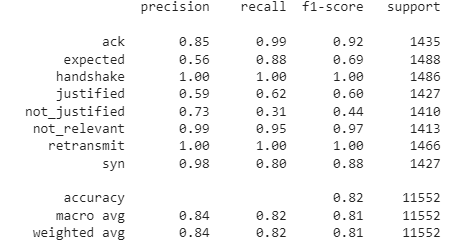
\includegraphics[width=\linewidth]{img/one_vs_rest_classifier.png}
        \caption{Report of one vs rest classifier.}
        \label{fig:one_vs_rest_classifier}
    \end{figure}
    It's clear how the classifier easly obtains an accurate precision for acknowledge, handshake, not\_relevant, retransmit and synchronization packets due to their easly identification by using the flags, the content type and the highest layer features. While for the application data packets (justified, not justified and expected) the classifier it's not able to easily identify the class due to the similar characteristics of these packets. Other problems related to this strategy comes from the definition of this kinf of classifier; since we create a single classifier for each class and the prediction happens by using a binary classification; there is an unbalanced distribution because the set of positives in much smaller than the positive ones.

    \textbf{One-vs-one}: the other possible strategy is one-vs-one; the implementation is quite similar to one-vs-rest approach but there is a difference on the reduction of the overall training set; it creates \(k (k-1)/2\) classifiers, where k is the number of existing classes, always by using an esimator object, and each of them recieves the samples of a pair of classes of the original training set and must learn to distinghuish these two calsses. At prediction time, all the \(k (k-1)/2\) classifiers will recieve an unseen sample and the class that recieves the highest number of votes will be predicted from the overall classifier.
    \begin{figure}[h!]
        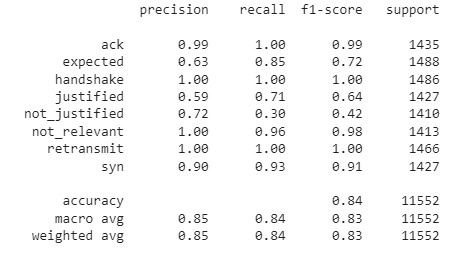
\includegraphics[width=\linewidth]{img/one_vs_one_classifier.png}
        \caption{Report of one vs one classifier.}
        \label{fig:one_vs_one_classifier}
    \end{figure}
    Here there is a better precision for the expected class but is not enough to say that this one is the best classifier.

    \subsubsection{Extension from binary}
    The other possible strategy to solve the problem of multiclass classification is using existing binary classifiers to solve multiclass problems.

    \textbf{Neural networks}: the main differences between neural networks for binary and multiclass classification are:
    \begin{itemize}
        \item \textbf{Output layer}: instead of using an output layer of just one neuron, we will use one neuron for each class. Another modification to apply on the output layer is the activation function, using the \textit{softmax} function (instead of \textit{sigmoid}) each neuron yields a probability for corresponding class.
        \item \textbf{Loss function}: instead of using \textit{binary\_crossentropy}, we will use the \textit{categorical\_crossentropy} that penalizes error in the probabilities predicted by a multiclass classifier (while the \textit{binary} does for binary classifier).
    \end{itemize}
    Once underlined the main differences we need to adapt the dataset to be compatible with the neural network; in particular we need to encode the label (classes) since neural network doesn't work with string but just with integer. First, using the class \textit{LabelEncoder} we map each label into an integer; then we create the relative matrix using the \textit{np\_utils.to\_categorical} method which, for each row, creates a list of 0, except for the position relative to the integer of the relative label. The method return a matrix composed of n row and m columns; where n is the number of samples and m is the number of classes.
    The sequential model used for the neural network is composed by four layers (one for input and one for output included). After different observations seems that 250 is the best number of epochs for our classifier.
    \begin{figure}[h!]
        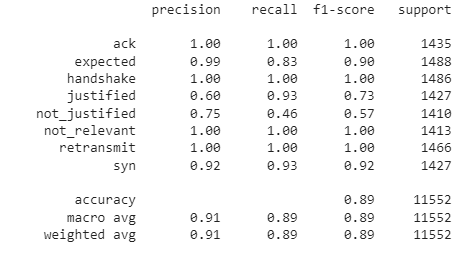
\includegraphics[width=\linewidth]{img/nn_classifier.png}
        \caption{Report of Neural Network classifier.}
        \label{fig:nn_classifier}
    \end{figure}
    The result highlights that till now the Neural Network classifier is better than the others. In particular, it shows a big difference between the expected and the not justified and justified packets; that is what we need for our purpose.

    \textbf{Naive Bayes}: this approach is based on the probability, there are different applications of Naive Bayes algorithm. Each of these application can be run without any parameter, but if a prior probability is defined, it will fit better. Kernel Density Estimation is a non-parametric way to estimate the probability density function of a random variable. We will use a Gaussian Naive Bayes classifier for our purpose.
    \begin{figure}[h!]
        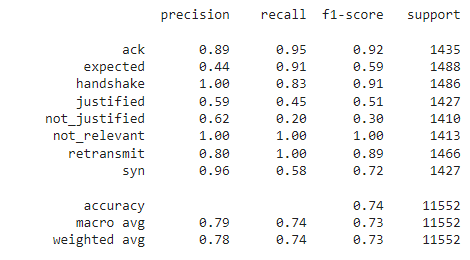
\includegraphics[width=\linewidth]{img/nb_classifier.png}
        \caption{Report of Naive Bayes classifier.}
        \label{fig:nb_classifier}
    \end{figure}
    It's clear how the results are worst than the Neural Network; this is also caused by the fact that Gaussian cannot work with negative values, which exist in our normalized dataset; the only accepted dataset is the original one, on which there is any kind of normalization technique.

    \textbf{Decision Trees}: the goal here is to create a model that predicts the value of a target variable by learning simple decision rules inferred from the data features. One application of Decision Tree is the Random Forest classifier, which fits a number of decision tree classifiers on various sub-samples of the dataset and uses averaging to improve the predictive accuracy and control over-fitting. We need to define the number of trees in the forest, by default it is set to 100 but after some experiments seems that 500 perform better.
In this case we can use the scaled dataset but in order to show the results a label parsing is needed (from string to integer).
    \begin{figure}[h!]
        \includegraphics[width=\linewidth]{img/decision_tree.png}
        \caption{Decision Tree classifier.}
        \label{fig:decision_tree}
    \end{figure}
The results seem to be better than the Neural Network, this behaviour is justified from the definition of the random forest; it tries to reduce the overfitting, that is really useful for our data (since we have variable length for the same kind of packets). The percentage of accuracy of the three application data packets it's increased and we can easily say that this is the best classifier for our purpose.

    \section{Conclusions}
    The aim of the project has been achieved; the results confirm the possibility to distinguish between different kind of packets. In particular, as introduced during the collection phase, both the justified and not justified packets shouldn't be sent from the Echo (the first ones because there is no motivation for the Echo to sent them also if it can record the voice due to the microphone status; while the second ones shouldn't be sent because the device is not listening the voice); a more accurate analysis on the nature of these packets can be done, may be possible that the packets sent when the device has microphone off are allowed since are simple synchronization packets without a clear pattern. Anyway, this study shows that there is a clear behaviour of the expected packets respect to the others; these packets have a lower payload length (seem that the Echo sent an huge amount of short length packets instead of small amount of long length when the communication is "authorized").
The final Random Forest classifier, together with a script that take into account the consideration done during the collection phase, can be applied on a proxy to block all the packets classified as justified and not justified and see if the Echo continues to work well or there is some configuration error.

    \bibliographystyle{plain}
    \bibliography{biblio_ref}

\end{document}
\endinput
%%
%% End of file `sample-sigconf.tex'.
